% !TeX program = pdflatex
% !TeX encoding = utf8
% !TeX spellcheck = uk_UA
% !BIB program = biber


\documentclass{LabWorkEng}
\usepackage[type=none]{fgruler}
\addbibresource{\jobname.bib}
\tikzset{
	magnet/.pic = {
		\fill [gray, draw=black] (-0.5,-0.25) rectangle (0.5,0.25);
	}
}


\title{Study of the of conservation laws of energy and linear momentum for collision of the balls}
\work{3}

\abstract{On the example of collision of balls check the conservation laws; calculate the energy dissipation coefficient and the mass correlation.}

\keywords{Total mechanical energy, linear momentum, conservation laws, collisions, absolutely elastic collision, absolutely inelastic  collision.}

\apparatus{experimental installation, to which the balls are fastened; set of balls of different weights and different materials; electronic stopwatch, scales.}

\begin{document}
\writedatatofile{\jobname}
\maketitle

\nocite{IrodovMechanics, BerkeleyMechanics, FLF1, Holyday}
\printbibliography

\section{Theoretibal background}

When moving, the bodies often collide each other. During the colission, both bodies are deformed, and as a result, the kinetic energy of the body before the collision, partially or completely transforms into the potential energy of the elastic deformation and the internal energy of the bodies. There are two limiting types of collision -- \textit{absolutely elastic} and \textit{absolutely inelastic}.

Consider these processes on an example of an elastic and inelastic collision in a one-dimensional space. This will greatly simplify mathematical calculations, without changing the essence. Simplification refers to the velocity, which in a one-dimensional space is a scalar. Of course, in general, velocity is a vector.

With a completely inelastic collision, one body stick to another one. In this case, the potential energy of deformation does not arise; kinetic energy is completely or partially converted into internal energy; after the collision, both bodies move at the same speed.

Suppose two bodies with masses $m_1$ and $m_2$ move towards each other (Fig.~\ref{inelcoll}) with velocities $v_1$ and $v_2$, respectively. After an inelastic collision, they form one body of net mass $m_1 + m_2$, which moves at a velocity $v$. From the linear momentum conservation law:
\begin{equation}\label{1}
	m_1v_1 - m_2v_2 = (m_1 + m_2)v
\end{equation}

\begin{figure}\centering
	\begin{picbox}	
	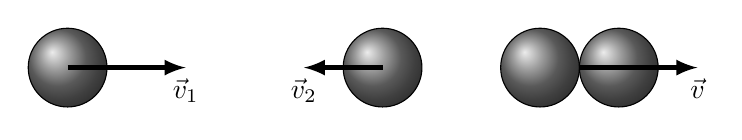
\begin{tikzpicture}
	\draw[ball color = gray] (0,0) circle (0.5);
	\draw[-latex, ultra thick] (0,0) -- +(1.5,0) node[below] {$\vec v_1$};
	\draw[ball color = gray] (4,0) circle (0.5);
	\draw[-latex, ultra thick] (4,0) -- +(-1,0) node[below] {$\vec v_2$};
	\draw[ball color = gray] (6,0) circle (0.5);\draw[ball color = gray] (7,0) circle (0.5);
	\draw[-latex, ultra thick] (6.5,0) -- +(1.5,0) node[below] {$\vec v$};	
	\end{tikzpicture}
	\end{picbox}	
	\caption{Inelastic collision}
	\label{inelcoll}
\end{figure}

From here we find the speed of the bodies after the collision:
\begin{equation}\label{2}
	v  = \frac{m_1v_1 - m_2v_2}{ m_1 + m_2}.
\end{equation}

In the case of an inelastic collision there is a law of conservation of momentum. Mechanical energy is not stored. Indeed, the total mechanical energy of the system before the collision (initial energy) is equal to the sum of the kinetic energies of each of the bodies:
\begin{equation}\label{3}
	E_\mathrm{initial} = \frac{1}{2}\left( {m_1v _1^2 + m_2v_2^2} \right).
\end{equation}
Mechanical energy after an collision (final energy) is defined as
\begin{equation}\label{4}
	E_\mathrm{final} = \frac{1}{2}\left( {{m_1} + {m_2}} \right){\upsilon ^2} = \frac{1}{2}\frac{{{{\left( {{m_1}{\upsilon _1} - {m_2}{\upsilon _2}} \right)}^2}}}{{{m_1} + {m_2}}}.
\end{equation}
When one writing the second equality in formula~\eqref{4}, we used the correlation~\eqref{2}. It is convenient to characterize the recoverment of mechanical energy using the coefficient $k$, which is defined as the ratio of $E_\mathrm{final}/E_\mathrm{initial}$. Taking into account~\eqref{3}, \eqref{4}, we obtain

\begin{equation}\label{5}
	k = \frac{E_\mathrm{final}}{E_\mathrm{initial}} = 1 - \frac{m_1m_2(v_1 + v_2)^2}{(m_1 + m_2)(m_1v_1^2 + m_2v_2^2)}.
\end{equation}

Formula~\eqref{5} indicates that the coefficient of mechanical energy recovery at a non-elastic collision is always less than one. In the case when one of the bodies, say, the first, before the collision was immovable (that is $v_1 = 0$), $k$ is determined only by the mass ratio of the bodies:
\begin{equation}\label{6}
	k = \frac{m_2}{m_1 + m_2}
\end{equation}
In the case of equal masses  ($m_1 = m_2$) and nonzero initial velocities:
\begin{equation}\label{6a}
	k = 1 - \frac{(v_1 + v_2)^2}{2( v_1^2 + v_2^2)}.
\end{equation}
and depends only on the initial velocities.

Is called an \textit{absolutely elastic collision}, in which the mechanical energy of the system is stored. When the elastic collision of the body first deformed and their kinetic energy passes into potential energy of elastic deformation. Then the bodies restore their shape and push away each other, while the energy of the elastic deformation again becomes kinetic. Body movement after elastic collision is determined by laws conservation of momentum and kinetic energy. Consider the central collision of two bodies moving toward each other with velocities $v_1$ and $v_2$ (Fig.~\ref{elcoll}). 

\begin{figure}\centering
	\begin{picbox}	
	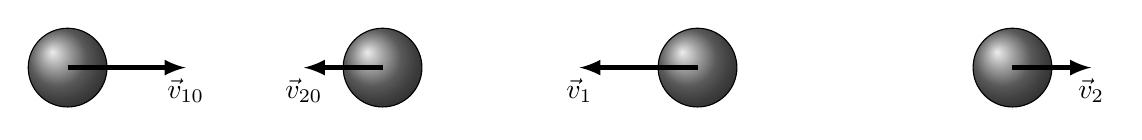
\begin{tikzpicture}
	\draw[ball color = gray] (0,0) circle (0.5);
	\draw[-latex, ultra thick] (0,0) -- +(1.5,0) node[below] {$\vec v_{10}$};
	\draw[ball color = gray] (4,0) circle (0.5);
	\draw[-latex, ultra thick] (4,0) -- +(-1,0) node[below] {$\vec v_{20}$};
	\begin{scope}[xshift=8cm]
	\draw[ball color = gray] (0,0) circle (0.5);
	\draw[-latex, ultra thick] (0,0) -- +(-1.5,0) node[below] {$\vec v_1$};
	\draw[ball color = gray] (4,0) circle (0.5);
	\draw[-latex, ultra thick] (4,0) -- +(1,0) node[below] {$\vec v_2$};	
	\end{scope}	
	\end{tikzpicture}
	\end{picbox}	
	\caption{Absolutely elastic collision}
	\label{elcoll}
\end{figure}

If the bodies move only translationally and do not rotate, then the equations of conservation of energy and momentum have the following form:
\begin{align}
	\frac{1}{2}\left( {{m_1}v_{10}^2 + {m_2}v_{20}^2} \right) &= \frac{1}{2}\left( {{m_1}v_1^2 + {m_2}v_2^2} \right), \label{7}\\
	{m_1}{v_{10}} - {m_2}{v_{20}} &=  - {m_1}{v_1} + {m_2}{v_2},\label{8}
\end{align}
where $v_1$ and $v_2$ -- body speed after the collision and it is believed that after the collision of the body move along the same line as before the collision. Rewrite equations~\eqref{7}, \eqref{8} in the following form:
\begin{align}
{m_1}\left( {{v_{10}} + {v_1}} \right)\left( {{v_{10}} - {v_1}} \right) &= {m_2}\left( {{v_{20}} + {v_2}} \right)\left( {{v_2} - {v_{20}}} \right) ,\label{7a}\\
{m_1}\left( {{v_{10}} + {v_1}} \right) &= {m_2}\left( {{v_{20}} + {v_2}} \right).\label{8a}
\end{align}

Comparing \eqref{7a} and \eqref{8a}, we arrive at the conclusion that
\begin{equation}\label{9}
	v_{10} - v_1 = v_2 - v_{20}.
\end{equation}

From~\eqref{8a} and \eqref{9} it is easy to determine the velocity of both bodies after the collision:
\begin{align}
	v_1 = \frac{\left( {{m_2} - {m_1}} \right){v_{10}} + 2m_2v_{20}}{m_1 + m_2}, \label{10} \\
	v_2 = \frac{\left( {m_1 - m_2} \right){v_{20}} + 2m_1v_{10}}{m_1 + m_2}. \label{10a}	
\end{align}

In the case when the first body before the collision was in a state of rest ($v_{10} = 0$), formula~\eqref{10} --~\eqref{10a} takes the form:
\begin{align}
v_1 = \frac{2m_2}{m_1 + m_2}{v_{20}}, \label{11}\\
v_2 = \frac{m_1 - m_2}{m_1 + m_2}{v_{20}}. \label{11a}
\end{align}

Formula~\eqref{11} -- \eqref{11a} indicates that in case of equal masses ($m_1 = m_2$) the bodies after the collision exchange of the speedes, namely, after the collision, the second body stops, and the first body moves with the speed $v_{20}$, which is the second body before the collision. The greater the difference between body masses, the less the speed of the first and the greater speed of the second body after the collision.

\section{Theoretical basis of the experiment}

Experimental installation is shown in Fig.~\ref{machine}. Two balls, $1$ and $2$, are suspended to a riser on  conducting threads of length $l$. In the bottom of  the riser there are two scales $3$ and $4$, by which the deviations of balls from the equilibrium position are measured.

\begin{figure}%{L}{0.5\linewidth}\centering
	\begin{subfigure}[t]{0.5\linewidth}\centering
		\begin{picbox}	
			\begin{tikzpicture}
			\pgfmathsetmacro{\angleshift}{5}
			\tikzstyle{ground}=[fill,pattern=north east lines,draw=none,minimum width=0.75cm,minimum height=0.3cm]
			\node (wall1) [ground, minimum width=3cm] {};
			\draw (wall1.north west) -- (wall1.north east);
			\fill[gray!50] (-0.1,0.3) rectangle (0.1,10);
			\node at (0,5.5) {\fgrulerdefnum{}\fgrulercaptioncm{}\ruler{upleft}{8cm}};
			\fill[gray] (-1,10) rectangle +(2,0.25);
			\draw (-0.25,10) -- +(0,-7.5) coordinate (A);
			\draw (0.25,10) -- node[above right] {$l$} ++(-90+\angleshift:7.5) coordinate (B);
			\draw[thick] (A) -- +(-90:0.5);
			\draw[thick] (B) -- +(-90+\angleshift:0.5);
			\node[ball color = gray, circle, minimum size=0.5cm,] at (A) {\tiny $1$};
			\node[ball color = gray, circle, minimum size=0.5cm,] at (B) {\tiny $2$};
			\fill[gray!50, draw = black] (-1,0.3) rectangle +(2,1);
			\fill[red] (-0.9,1) rectangle +(0.3,0.1);
			\fill[black] (-0.9,0.8) rectangle +(0.3,0.1);
			\fill[black] (-0.9,0.6) rectangle +(0.3,0.1);
			\draw[fill=white] (-0.5,0.6) rectangle node[text = red] {time} +(1.3,0.5);
			\fill[black] (-0.9,0.15) rectangle +(0.3,0.15);
			\fill[black] (0.6,0.15) rectangle +(0.3,0.15);
			\fill[gray!20, draw = black] (-2,1.5) coordinate (S1) -- +(1.5,0) coordinate (A) -- +(0,0.5) coordinate (B) -- cycle;
			\fill[gray!20, draw = black] (2,1.5) -- +(-1.5,0) coordinate (S2) -- +(0,0.5) -- cycle;
			\node at ([shift={(0.5,0.15)}]S1) {\tiny $3$};
			\node at ([shift={(1,0.15)}]S2) {\tiny $4$};
			\coordinate (M) at (1.7,2.8);
			\pic[rotate = 18] at (M) {magnet};
			\node at (M) {\tiny $5$};
			\end{tikzpicture}
		\end{picbox}
		\subcaption{Experimental installation.}
		\label{machine}
	\end{subfigure}
	\begin{subfigure}[t]{0.5\linewidth}\centering
	\begin{picbox}	
		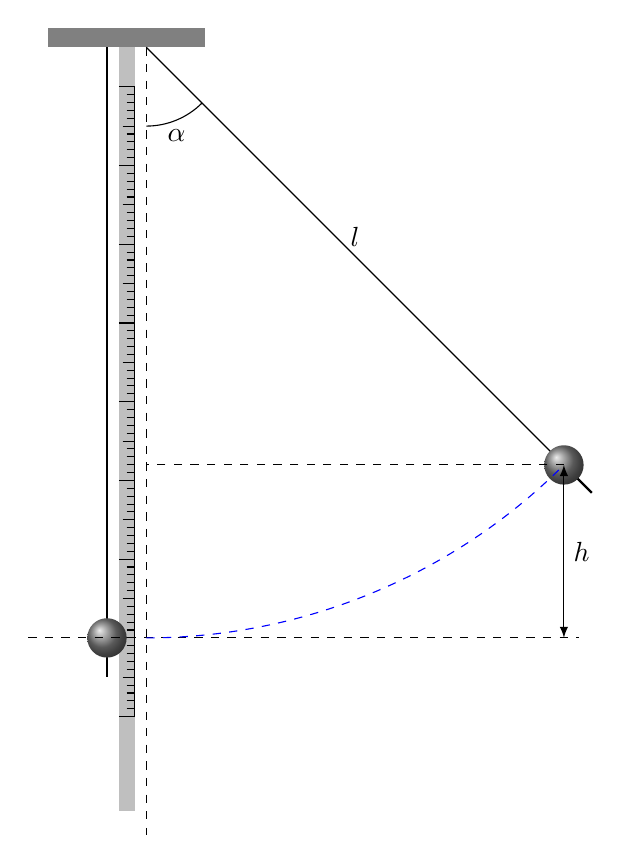
\begin{tikzpicture}
		\pgfmathsetmacro{\angleshift}{45}
		\fill[gray!50] (-0.1,0.3) rectangle (0.1,10);
		\node at (0,5.5) {\fgrulerdefnum{}\fgrulercaptioncm{}\ruler{upleft}{8cm}};
		\fill[gray] (-1,10) rectangle +(2,0.25);
		\draw (-0.25,10) -- +(0,-7.5) coordinate (A);
		\draw (0.25,10) -- node[above] {$l$} ++(-90+\angleshift:7.5) coordinate (B);
		\draw[thick] (A) -- +(-90:0.5);
		\draw[thick] (B) -- +(-90+\angleshift:0.5);
		\node[ball color = gray, circle, minimum size=0.5cm] at (A) {};
		\node[ball color = gray, circle, minimum size=0.5cm] at (B) {};
		\draw[dashed] ([xshift=-1cm]A) -- ([xshift=6cm]A) coordinate (P);
		\draw[dashed] (0.25,10) -- +(0,-10);
		\draw[] (0.25,10) +(0,-1)  arc (-90:-90+\angleshift:1) node[pos=0.5, below] {$\alpha$};
		\draw[dashed, blue] (0.25,10) +(0,-7.5) coordinate (F)  arc (-90:-90+\angleshift:7.5);
		\draw[latex-latex] (B) -- node[right] {$h$} ({B|-P});
		\draw[dashed] (B) -- (F|-B);		
%		\fill[gray!50, draw = black] (-1,0.3) rectangle +(2,1);
%		\fill[red] (-0.9,1) rectangle +(0.3,0.1);
%		\fill[black] (-0.9,0.8) rectangle +(0.3,0.1);
%		\fill[black] (-0.9,0.6) rectangle +(0.3,0.1);
%		\draw[fill=white] (-0.5,0.6) rectangle node[text = red] {time} +(1.3,0.5);
%		\fill[black] (-0.9,0.15) rectangle +(0.3,0.15);
%		\fill[black] (0.6,0.15) rectangle +(0.3,0.15);
%		\fill[gray!20, draw = black] (-2,1.5) -- +(1.5,0) coordinate (A) --   +(0,0.5) coordinate (B) -- cycle;
%		\fill[gray!20, draw = black] (2,1.5) -- +(-1.5,0) -- +(0,0.5) -- cycle;
		\end{tikzpicture}
	\end{picbox}
	\subcaption{Calculation of the ball's lifted height.}
	\label{theory}
	\end{subfigure}
\end{figure}

At the beginning of the experiment, the ball $1$ is in equilibrium, and the ball $2$ is deviated at an angle $\alpha$ from the vertical axis and fixed with the help of an electromagnet $5$. After the electromagnet is switched off, ball $2$ begins to move (initial ball speed is zero). The velocity of the ball $2$ before the collision is determined at the initial angle of deviation $\alpha$, based on the law of conservation of mechanical energy.

\begin{equation}\label{12}
	mgh = \frac{1}{2}mv_{20}^2
\end{equation}
where $h$ -- height at which the ball was lifted, $g$ -- acceleration of free fall, $v_{20}$ -- the velocity of the ball $2$ at the point of equilibrium. For geometric reasons (See Fig.~\ref{theory}):

\begin{equation}\label{13}
	h = l(1 - \cos \alpha) = 2l{\sin ^2}\frac{\alpha }{2}
\end{equation}

Thus, if the maximum angle of deviation of a ball is equal to $\alpha$ then its velocity at the equilibrium point is determined by the formula:
\begin{equation}\label{14}
	v_{20} = 2\sqrt{gl} \sin\frac{\alpha}{2}.
\end{equation}

Similarly, by measuring the angle of deviation of the ball $1$, we can find its velocity $v_{20}$ immediately after the collision.

In the theoretical guide, we considered two limiting cases of an absolutely elastic and absolutely inelastic impact. In real experiments, during impact, energy is partially dissipated. In this paper, the energy dissipation coefficient $\beta$, which is defined as the ratio of energy loss during impact with the initial energy, is measured:
\begin{equation}\label{15}
	\beta  = \frac{E_\mathrm{initial} - E_\mathrm{final}}{E_\mathrm{initial}}.
\end{equation}

Consider the case when the first ball before the impact is at rest ($v_{20} = 0$). Then the laws of conservation of energy and momentum~\eqref{7}, \eqref{8} taking into account~\eqref{15} will look like:
\begin{align}
	( 1 - \beta )m_2v_{20}^2 = m_1v_1^2 + m_2v_2^2, \label{16}\\
	m_2v_{20} = m_1v_1 - m_2v_2. \label{17}
\end{align}
(in the formula~\eqref{17} the modules of velocities are inserted!).

An experimental setup allows you to measure $v_{20}$ and $v_1$ speeds. Consequently, by excluding from equations~\eqref{16}, \eqref{17} $v_2$, we can find the coefficient $\beta$. For identical balls:

\begin{equation}\label{18}
	\beta  = \frac{{2{v_1}\left( {v_{20} - v_1} \right)}}{{v_{20}^2}} = 2R\left( {1 - R} \right), \, R = \frac{v_1}{v_{20}}
\end{equation}


On the other hand, according to the known coefficient $\beta$ of equations~\eqref{16}, \eqref{17} we can find the relation of the masses of the impacting balls. Indeed, solving these equations for $v_2$, $m_1/m_2$ we obtain:
\begin{equation}\label{19}
	\frac{{{m_1}}}{{{m_2}}} = \frac{{2 - R \pm \sqrt {{{\left( {2 - R} \right)}^2} - 4\beta } }}{{2R}}.
\end{equation}

\section{Experimental details}

The electromagnet is switched off by pressing the \tcbox{\sc{Reset}} button. In the intervals between experiments, it is desirable to switch off the electromagnet!

The time of contact of the balls is fixed by an electronic stopwatch, which is attached to the electrical circuit formed by balls and threads of the suspension. When impact balls electrical circuit is closed and the stopwatch is triggered.

\section{Tasks}

\begin{enumerate}
	\item Take two steel balls with the same numbers. Weigh them and carefully fasten them on the hanging. Ensure that the contact is impact-centered.
	\item Deviate the ball $2$ (Fig. 4.3.) to some angle and release. Measure the angle of deviation of the ball $1$ after the first impact. Measurement should be repeated at least $10$ times.
	\item Repeat measurement for point $2$ for different initial angles of deviation of the ball (we recommend $5^\circ$, $10^\circ$, $15^\circ$).
	\item Repeat steps $2$, $3$ for another pair of identical balls (you only need to explore three pairs of balls).
	\item Take a couple of balls with different numbers. Weigh them. Repeat steps $2$ and $3$. Why do you think the balls have different and identical numbers?
	\item 	Select two more pairs of balls with different numbers and repeat experiment $5$. So you have to get data for $6$ pairs of balls at the three angles for each pair (only $18$ measurements of the angle of deviation).
	\item Think about what kind of mistakes make the devices? Can they evaluate how to do it? What are they: random or systematic?
\end{enumerate}

\section*{Control questions}

\begin{enumerate}
	\item What are elastic and inelastic collisions?
	\item Formulate and derive the laws of conservation of momentum and total mechanical energy for elastic and inelastic collisions. In what conditions these laws can not be applied?
	\item What are central and noncentral collisions? Explain how the balls will move for a noncentral collision.
	\item Calculate the fraction of the energy of the balls passing into the internal energy during an inelastic collision, using the results of the laboratory work.
%	\item Suppose the mass of one of the balls is much larger than the mass of the second ball. Determine the velocities of the balls after a completely elastic collision, if at the beginning of the experiment in the rest was: a) a lighter ball; b) a heavier ball. %Determine the proportion of the transmitted momentum and energy in comparison with the initial values in both cases.
	\item How precisely are the laws of conservation of momentum and mechanical energy in the experiments carried out? What leads to deviations from conservation laws?
%	\item In your opinion, are the errors of the experiments performed on the size of the balls? What difficulties will arise if you increase the size of the balls? And if you reduce it?
\end{enumerate}


\end{document}